\documentclass[11pt,a4paper]{article}

\usepackage[utf8]{inputenc}
\usepackage[margin=2.5cm]{geometry}
\usepackage{amsmath,amssymb}
\usepackage{graphicx}
\usepackage{booktabs}
\usepackage{enumitem}
\usepackage{hyperref}
\usepackage{natbib}
\usepackage{tikz}
\usetikzlibrary{arrows.meta,positioning,fit,backgrounds,calc}
\usepackage{xcolor}

\definecolor{memblue}{HTML}{DBEAFE}
\definecolor{trustorange}{HTML}{FED7AA}
\definecolor{beliefgreen}{HTML}{D1FAE5}
\definecolor{envpink}{HTML}{FCE7F3}
\definecolor{commpurple}{HTML}{EDE9FE}
\definecolor{normyellow}{HTML}{FEF9C4}
\definecolor{lockinpink}{HTML}{F5D0FE}
\definecolor{normred}{HTML}{FECACA}

\title{\textbf{Dual-Memory Cognitive Lock-in:\\Norm Emergence Through Experience, Trust, and Normative Constraint}}
\author{}
\date{}

\begin{document}
\maketitle

\begin{abstract}
We present a dual-memory model of norm emergence in coordination games. Agents maintain two qualitatively distinct memory systems: an \emph{experience memory} that tracks interaction history through a trust-modulated sliding window, and a \emph{normative memory} that stores internalised rules as decision constraints. The two systems are bridged by a single state variable---trust---which plays three natural roles: it controls the experience memory window (cognitive lock-in), determines susceptibility to norm internalisation (low trust $\to$ accept external rules), and governs whether norm violations trigger enforcement or belief updating (high trust $\to$ enforce; low trust $\to$ update). Norm formation follows a drift-diffusion process grounded in \citet{germar2014social}: uncertain agents accumulate stochastic evidence from observing consistent behaviour until a crystallisation threshold is crossed. Norm enforcement is violation-triggered and confidence-dependent, consistent with \citet{fehr2002altruistic} and \citet{toribio2023proof}. The three feedback loops of the model---individual learning, social amplification, and normative pressure---emerge naturally from the dual-memory architecture without requiring separate mechanisms.
\end{abstract}

% =====================================================================
\section{Introduction}
% =====================================================================

Starting from a cold start---50-50 random strategy distribution, no shared history---how does randomness become a social norm? Not merely behavioural convergence, but a self-enforcing pattern sustained by mutual expectations \citep{bicchieri2006grammar}.

The question has two parts: (1) how do norms \emph{form}, and (2) how do norms \emph{persist}? Existing models typically address these through a single mechanism---imitation, best response, or conformist transmission. We argue that formation and persistence involve \emph{qualitatively different cognitive processes}, served by different memory systems:

\begin{itemize}[itemsep=2pt]
    \item \textbf{Experience memory}: a statistical system that tracks what happened and forms beliefs. It answers ``what \emph{is} the pattern?''
    \item \textbf{Normative memory}: a rule-based system that stores internalised constraints. It answers ``what \emph{should} I do?''
\end{itemize}

The is--ought gap \citep{hume1739treatise} means that norms cannot be derived from experience alone. An agent who observes that 70\% of partners play strategy~$A$ has an empirical belief, not a norm. The transition from ``most people do $A$'' to ``one \emph{should} do $A$'' requires a qualitatively different cognitive step.

We propose that this step is \textbf{norm internalisation}: the process by which an uncertain agent, observing confident and consistent behaviour in others, infers the existence of a rule and adopts it as a decision constraint. Trust---the agent's confidence in the predictability of the social environment---is the single variable that bridges the two memory systems, governing when agents learn from experience, when they internalise norms, and when they enforce them.

% =====================================================================
\section{Model Overview}
% =====================================================================

\subsection{Environment}

\begin{itemize}[itemsep=2pt]
    \item $N$ agents (even), strategy set $S = \{A, B\}$
    \item Pure coordination game: payoff 1 if both choose same strategy, 0 otherwise
    \item Each time step $t$: agents randomly paired, simultaneous strategy choice
    \item Agents observe partner's strategy (anonymous); additionally observe $k$ random interactions
\end{itemize}

\subsection{Agent State}

Each agent $i$ at time $t$ maintains:

\begin{table}[h]
\centering
\begin{tabular}{llll}
\toprule
\textbf{Component} & \textbf{Symbol} & \textbf{Type} & \textbf{Role} \\
\midrule
Trust & $T_i(t) \in [0, 1]$ & State variable & Bridges both memories \\
Experience memory & $M_i^E(t)$ & FIFO queue & Statistical belief formation \\
Normative memory & $M_i^N$ & Rule + strength + anomalies & Decision constraint \\
\bottomrule
\end{tabular}
\end{table}

\subsection{Architectural Principle}

Trust is \textbf{not} a parameter of either memory system. It is a single variable whose meaning naturally produces three roles:

\begin{center}
\begin{tabular}{lll}
\toprule
\textbf{Trust level} & \textbf{Meaning} & \textbf{Consequence} \\
\midrule
Low ($< 0.3$) & ``I am uncertain'' & Short window; susceptible to norm internalisation \\
Medium ($0.3$--$0.7$) & ``I roughly know'' & Moderate window; follows existing norm \\
High ($> 0.7$) & ``I am confident'' & Long window; can override or enforce norm \\
\bottomrule
\end{tabular}
\end{center}

% =====================================================================
\section{Experience Memory and Cognitive Lock-in}
% =====================================================================

Experience memory is the statistical layer. It stores direct interaction records and (optionally) observation data, producing a belief distribution over strategies.

\subsection{Belief Formation}

\begin{equation}
b_A = \frac{n_A}{|M'^E_i(t)|}, \quad b_B = 1 - b_A
\end{equation}
where $n_A$ is the count of strategy $A$ in the effective window. Default: $[0.5, 0.5]$.

\subsection{Action Selection (Probability Matching)}

\begin{equation}\label{eq:prob_matching}
P(s_i = A) = b_A^{\text{eff}}, \quad P(s_i = B) = b_B^{\text{eff}}
\end{equation}
where $\mathbf{b}^{\text{eff}}$ is the effective belief after normative constraint (Section~\ref{sec:decision}).

\subsection{Trust Update}

\begin{equation}\label{eq:trust_update}
T_i(t\!+\!1) = \begin{cases}
T_i(t) + \alpha (1 - T_i(t)) & \text{if prediction correct} \\
T_i(t) (1 - \beta) & \text{if prediction wrong}
\end{cases}
\end{equation}

Asymmetric by design \citep{slovic1993perceived}: trust builds slowly (additive, saturating) and breaks quickly (multiplicative). Steady state:
\begin{equation}\label{eq:trust_steady}
T^* = \frac{p\alpha}{p\alpha + (1-p)\beta}
\end{equation}

\subsection{Trust--Memory Window Linkage}

\begin{equation}\label{eq:window}
w_i(t) = \text{base} + \lfloor T_i(t) \times (\text{max} - \text{base}) \rfloor
\end{equation}

The upper bound $\text{max} = 6$ follows \citet{hertwig2010decisions} and \citet{nevo2012bi}, whose BI-SAW model---winner of the 2010 Market Entry Prediction Competition---found that agents recall only the most recent 6 trials.

\subsection{The Cognitive Lock-in Mechanism}

\begin{center}
Majority forms (drift) $\to$ prediction accuracy $\uparrow$ $\to$ trust $\uparrow$ $\to$ window $\uparrow$ $\to$ beliefs stabilise $\to$ norm resilience $\uparrow$
\end{center}

Probability matching is behaviourally neutral: any norm emergence is attributable to the memory mechanism, not behavioural biases. \textbf{Limitation}: convergence is slow without social amplification.

% =====================================================================
\section{Normative Memory}
% =====================================================================

Normative memory is qualitatively different from experience memory. It stores a \emph{rule}, not data. It acts as a \emph{constraint} on decisions, not a source of beliefs.

\subsection{Structure}

\begin{equation}
M_i^N = \left(\, r_i \in S \cup \{\varnothing\},\;\; \sigma_i \in [0,1],\;\; a_i \in \mathbb{N},\;\; e_i \in \mathbb{R} \,\right)
\end{equation}

\begin{itemize}[itemsep=2pt]
    \item $r_i$: the norm (which strategy is ``the rule''), or $\varnothing$ if no norm has formed
    \item $\sigma_i$: norm strength (how constraining the rule is)
    \item $a_i$: anomaly count (accumulated violations observed)
    \item $e_i$: DDM evidence accumulator (pre-crystallisation)
\end{itemize}

Normative memory is \textbf{not FIFO}. It does not slide, decay, or reweight. Once formed, the norm persists as a discrete rule until overthrown through crisis.

\subsection{Norm Formation: Drift-Diffusion Crystallisation}\label{sec:formation}

Norm formation follows a drift-diffusion process \citep{germar2014social,germar2019learning}. Observations accumulate as noisy evidence; a norm crystallises when accumulated evidence crosses a threshold.

\paragraph{Theoretical basis.} \citet{germar2014social} showed that social norms alter the drift rate in perceptual decision-making. \citet{germar2019learning} demonstrated that this alteration \emph{persists} after social influence is removed---norms are internalised as a persistent cognitive bias, not a transient effect. \citet{tenenbaum2011grow} established that rule learning from examples is fundamentally probabilistic (Bayesian inference over rule hypotheses).

\paragraph{Mechanism.} At each tick, if $r_i = \varnothing$ (no norm yet):

\begin{align}
\text{drift}_i &= (1 - T_i) \times \text{consistency}(\text{observations}) \label{eq:drift} \\
e_i(t\!+\!1) &= \max\!\big(0,\; e_i(t) + \text{drift}_i + \mathcal{N}(0, \sigma_{\text{noise}}^2)\big) \label{eq:ddm} \\
\text{If } e_i &> \theta_{\text{crystal}}: \quad r_i \leftarrow s^*,\;\; \sigma_i \leftarrow \sigma_0,\;\; a_i \leftarrow 0 \label{eq:crystal}
\end{align}

where $\text{consistency} = \max(f_A, f_B)$ over observed strategies, $s^*$ is the dominant observed strategy, and $\theta_{\text{crystal}}$ is the crystallisation threshold.

\paragraph{Properties.}
\begin{itemize}[itemsep=2pt]
    \item \textbf{Not deterministic}: noise makes the exact crystallisation moment stochastic, creating individual variation \citep{sanborn2016bayesian}
    \item \textbf{Not purely statistical}: the norm is a discrete rule, not a probability distribution; evidence accumulates toward a phase transition, not a gradual belief update
    \item \textbf{Trust-gated}: low trust $\to$ high drift rate (uncertain agents absorb norm evidence faster); high trust $\to$ low drift rate (confident agents resist norm formation because they trust their own experience)
    \item \textbf{Grounded in ``copy when uncertain''} \citep{rendell2010copy}: agents internalise norms \emph{precisely when} their own experience is unreliable
\end{itemize}

\paragraph{Why does a norm form?} The ``should'' does not emerge from the agent's own experience. It is \emph{inferred} from the contrast between the agent's uncertainty and others' consistency \citep{sherif1936psychology,deutsch1955study}:
\begin{quote}
    ``They are so consistent, they must know something I don't. That must be the rule.''
\end{quote}

No agent needs to explicitly ``send'' a normative signal. The first norms are inferred from observed behavioural consistency---a natural byproduct of cognitive lock-in producing high-trust, high-consistency agents.

\subsection{Norm Maintenance: Anomaly Accumulation}

Once $r_i \neq \varnothing$, the norm is maintained by anomaly tracking, not statistical updating:

\begin{equation}\label{eq:anomaly}
\text{If } s^*_{\text{observed}} \neq r_i: \quad a_i \leftarrow a_i + 1
\end{equation}

Observations \emph{consistent} with the norm cause nothing---they are ``normal.'' This is the key non-statistical property: 99 conforming observations and 1 violation $\neq$ ``norm strength = 0.99.'' The 1 violation is an anomaly, not a data point for updating.

\subsection{Norm Overthrow: Crisis and Phase Transition}

\begin{equation}\label{eq:crisis}
\text{If } a_i \geq \theta_{\text{crisis}}: \quad \sigma_i \leftarrow \sigma_i \times \lambda_{\text{crisis}}, \quad a_i \leftarrow 0
\end{equation}

When anomalies accumulate past $\theta_{\text{crisis}}$, norm strength drops sharply (not gradually). If $\sigma_i < \sigma_{\min}$:

\begin{equation}
r_i \leftarrow \varnothing, \quad e_i \leftarrow 0 \quad \text{(norm dissolved; open to re-crystallisation)}
\end{equation}

This mirrors Kuhn's (\citeyear{kuhn1962structure}) paradigm shifts: normal science tolerates anomalies until a crisis threshold triggers revolution.

% =====================================================================
\section{Decision Integration}\label{sec:decision}
% =====================================================================

When a norm exists, it constrains the experience-based belief:

\begin{align}
\text{compliance}_i &= (1 - T_i)^k, \quad k > 1 \label{eq:compliance} \\
\mathbf{b}^{\text{norm}} &= \text{one\_hot}(r_i) \label{eq:norm_belief} \\
\mathbf{b}^{\text{eff}}_i &= \text{compliance}_i \cdot \mathbf{b}^{\text{norm}} + (1 - \text{compliance}_i) \cdot \mathbf{b}^{\text{exp}}_i \label{eq:effective}
\end{align}

The exponent $k > 1$ creates a nonlinear threshold: compliance drops slowly at first and rapidly only at very high trust. With $k = 2$:

\begin{center}
\begin{tabular}{ccc}
\toprule
Trust $T$ & Compliance $(1-T)^2$ & Behaviour \\
\midrule
0.3 & 0.49 & Mostly follows norm \\
0.5 & 0.25 & Norm still constrains \\
0.7 & 0.09 & Experience dominates \\
0.9 & 0.01 & Essentially free of norm \\
\bottomrule
\end{tabular}
\end{center}

When $r_i = \varnothing$: $\mathbf{b}^{\text{eff}}_i = \mathbf{b}^{\text{exp}}_i$ (pure experience-based decision).

% =====================================================================
\section{Norm Enforcement: Violation-Triggered Signalling}
% =====================================================================

\subsection{When Do Agents Signal?}

Norm enforcement is \textbf{reactive}, not proactive. An agent broadcasts a normative signal only when three conditions hold simultaneously:

\begin{enumerate}[itemsep=2pt]
    \item The agent \textbf{has a norm} ($r_i \neq \varnothing$)
    \item The agent \textbf{is confident} ($T_i > \theta_{\text{enforce}}$)
    \item The agent \textbf{observes a violation} ($s^*_{\text{observed}} \neq r_i$)
\end{enumerate}

\paragraph{Theoretical basis.}
\begin{itemize}[itemsep=2pt]
    \item \citet{fehr2002altruistic}: punishment is triggered by observed defection, costly, and directed at violators
    \item \citet{fehr2004third}: 60\% of uninvolved third parties punish norm violations
    \item \citet{toribio2023proof}: across six studies, ambiguity about whether a violation occurred \emph{significantly reduces} punishment. Certainty is a prerequisite for enforcement.
    \item \citet{skitka2010moral}: moral conviction predicts willingness to enforce and resistance to conformity pressure
\end{itemize}

\subsection{Asymmetric Response to Violations}

The same observed violation produces qualitatively different responses depending on the observer's trust:

\begin{equation}\label{eq:violation_response}
\text{Observe } s^* \neq r_i: \quad \begin{cases}
T_i > \theta_{\text{enforce}}: & \text{broadcast}(r_i) \quad \textit{(``He is wrong''---enforce)} \\
T_i \leq \theta_{\text{enforce}}: & a_i \leftarrow a_i + 1 \quad \textit{(``Maybe the rule changed''---update)}
\end{cases}
\end{equation}

\paragraph{Theoretical basis.}
\begin{itemize}[itemsep=2pt]
    \item Uncertain agents \emph{update}: \citet{sherif1936psychology} showed that uncertain individuals converge toward others' judgments. \citet{deutsch1955study} established that uncertainty activates informational influence (learning mode). \citet{cialdini2004social}: uncertainty drives norm-seeking behaviour.
    \item Confident agents \emph{enforce}: \citet{skitka2010moral} showed that moral conviction produces enforcement and resistance to conformity. \citet{fehr2000cooperation}: high contributors (most committed) punish most. \citet{chudek2011culture}: norm psychology follows a sequence---infer $\to$ internalise $\to$ enforce. Enforcement requires prior internalisation.
\end{itemize}

This dual response is a \textbf{novel contribution} of our model, synthesising across the conformity, punishment, and moral conviction literatures. It has not been tested in a single experiment but follows as a natural prediction from convergent evidence.

\subsection{Effect of Normative Signals on Receivers}

Receiving a normative signal amplifies the DDM drift rate for norm formation (Eq.~\ref{eq:drift}):

\begin{equation}\label{eq:signal_boost}
\text{drift}_i^{\text{signal}} = (1 - T_i) \times \text{consistency} \times \gamma_{\text{signal}}, \quad \gamma_{\text{signal}} > 1
\end{equation}

A normative signal is stronger than a behavioural observation because it carries explicit prescriptive content (``you \emph{should} do $X$''), not merely descriptive information (``someone did $X$'').

% =====================================================================
\section{Observations: The Dual-Purpose Channel}
% =====================================================================

Observations are processed by \textbf{both} memory systems simultaneously, not routed exclusively to one:

\begin{enumerate}[itemsep=2pt]
    \item \textbf{Experience memory}: observations are additional data points, updating the belief distribution (statistical processing)
    \item \textbf{Normative memory}: the same observations are checked for consensus (rule detection)
    \begin{itemize}
        \item If $r_i = \varnothing$: consistency feeds the DDM evidence accumulator (Eq.~\ref{eq:ddm})
        \item If $r_i \neq \varnothing$: violations increment the anomaly counter (Eq.~\ref{eq:anomaly})
    \end{itemize}
\end{enumerate}

The two systems extract different information from identical observations: experience memory extracts \emph{frequencies}; normative memory detects \emph{consensus} (or violations of it).

% =====================================================================
\section{Three Emergent Feedback Loops}
% =====================================================================

The dual-memory architecture produces three feedback loops without requiring separate mechanisms for each:

\subsection{Loop 1: Cognitive Lock-in (Experience Memory)}

\begin{center}
Correct prediction $\to$ $T \!\uparrow$ $\to$ window $\uparrow$ $\to$ beliefs stabilise $\to$ better predictions
\end{center}

\textbf{Source}: experience memory + trust update. Operates through cognition, not behaviour.

\textbf{References}: \citet{slovic1993perceived} (asymmetric trust); \citet{behrens2007learning} (volatility-adjusted learning rate).

\subsection{Loop 2: Social Amplification (Observations)}

\begin{center}
High-trust agents behave consistently $\to$ observed by others $\to$ others' experience beliefs shift $\to$ more coordination $\to$ trust rises faster
\end{center}

\textbf{Source}: observations feeding experience memory. Amplifies both positive and negative feedback.

\textbf{References}: \citet{toyokawa2019conformist} (conformist social learning); \citet{henrich1998conformist} (conformist transmission).

\subsection{Loop 3: Normative Pressure (Emergent)}

\begin{center}
High-trust agents behave consistently $\to$ low-trust agents observe consensus $\to$ DDM evidence accumulates $\to$ norms crystallise $\to$ agents follow norms $\to$ more consistency $\to$ agents gain trust $\to$ agents observe violations and \textbf{enforce} $\to$ enforcement accelerates others' DDM $\to$ cascade
\end{center}

\textbf{Source}: observations feeding normative memory (DDM) + violation-triggered enforcement. This loop \emph{emerges} from the dual-memory architecture---it is not a separate mechanism.

\textbf{Key property}: Loop 3 is the only loop that produces \emph{social norms} in the sense of \citet{bicchieri2006grammar}. Without normative memory, the model produces conventions (Loops 1+2 only). With normative memory, the model produces norms with prescriptive force.

\textbf{References}: \citet{fehr2002altruistic} (violation-triggered enforcement); \citet{centola2018tipping} (tipping point cascade); \citet{chudek2011culture} (infer $\to$ internalise $\to$ enforce sequence).

\subsection{Loop Interaction}

\begin{center}
\begin{tabular}{lccc}
\toprule
& \textbf{Loop 1} & \textbf{Loop 2} & \textbf{Loop 3} \\
& Cognitive lock-in & Social amplification & Normative pressure \\
\midrule
Memory system & Experience & Experience & Normative \\
Drives & Stability & Speed & Norm emergence \\
Mechanism & Window $= f(T)$ & Observation $\to$ belief & DDM $\to$ rule $\to$ enforcement \\
Feedback type & Reinforcing + balancing & Amplifier (both) & Positive with threshold \\
Without it & Slow convergence & No acceleration & Conventions only \\
\bottomrule
\end{tabular}
\end{center}

% =====================================================================
\section{Norm Emergence Phases from Cold Start}
% =====================================================================

\subsection{Detection Levels}

\begin{table}[h]
\centering
\small
\begin{tabular}{clll}
\toprule
\textbf{Level} & \textbf{Name} & \textbf{Condition} & \textbf{Threshold} \\
\midrule
0 & \textsc{None} & No regularity & majority $< 0.70$ \\
1 & \textsc{Behavioral} & Behavioural regularity & $\geq 0.95$ for 50 ticks \\
2 & \textsc{Empirical} & + Accurate empirical expectations & belief error $< 0.10$ \\
3 & \textsc{Shared} & + Belief consensus & belief variance $< 0.05$ \\
4 & \textsc{Normative} & + Normative rule internalised & $\geq 80\%$ agents have $r_i \neq \varnothing$ \\
5 & \textsc{Institutional} & + Self-enforcing stability & maintained 200+ ticks \\
\bottomrule
\end{tabular}
\end{table}

Level 4 requires normative memory; Level 5 additionally requires violation-triggered enforcement (Loop~3 active).

\subsection{Emergence Timeline}

\paragraph{Phase 1: Random drift (ticks 0--30).}
50-50, no consensus. Trust declining (predictions $\approx$ random). Short memory windows. Negative feedback dominates. Normative DDM accumulators near zero. Level: \textsc{None}.

\paragraph{Phase 2: Symmetry breaking (ticks 30--80).}
Random drift creates a small majority (55--65\%). Trust stabilises for majority agents. Observations begin showing bias. DDM evidence starts accumulating in low-trust agents. Level: approaching \textsc{Behavioral}.

\paragraph{Phase 3: Norm crystallisation (ticks 80--150).}
First norms crystallise (DDM crosses threshold) in the most uncertain agents. These agents start following the norm $\to$ more behavioural consistency. Simultaneously, trust rises for consistent agents. Level: \textsc{Behavioral} achieved.

\paragraph{Phase 4: Enforcement onset (ticks 150--250).}
Agents who internalised norms early have now gained trust through successful coordination. They cross $\theta_{\text{enforce}}$ and begin broadcasting normative signals when violations are observed. These signals accelerate DDM in remaining agents (Eq.~\ref{eq:signal_boost}). Positive cascade. Level: \textsc{Empirical} $\to$ \textsc{Shared} $\to$ \textsc{Normative}.

\paragraph{Phase 5: Institutional stability (ticks 250+).}
Nearly all agents have norm $+$ high trust. Violations are rare and immediately enforced. Anomaly counts stay low. The norm is self-sustaining. Level: \textsc{Institutional}.

% =====================================================================
\section{Experimental Design}
% =====================================================================

\subsection{2$\times$2 Factorial}

\begin{table}[h]
\centering
\begin{tabular}{lcc}
\toprule
& \textbf{Experience Only} & \textbf{Dual Memory} \\
\midrule
\textbf{Fixed Window} & Baseline & Normative constraint only \\
\textbf{Dynamic Window} & Cognitive lock-in & Full model \\
\bottomrule
\end{tabular}
\end{table}

\subsection{Predictions}

\begin{itemize}[itemsep=2pt]
    \item \emph{Baseline}: Slowest. Max level: \textsc{Behavioral}.
    \item \emph{Normative only}: Norms can form but no lock-in stability. Max: \textsc{Normative} but fragile.
    \item \emph{Lock-in only}: Stable but slow; conventions not norms. Max: \textsc{Shared}.
    \item \emph{Full model}: Fastest and most stable. Max: \textsc{Institutional}.
\end{itemize}

% =====================================================================
\section{Testable Hypotheses}
% =====================================================================

\begin{description}[style=nextline]
    \item[H1: Norm formation is stochastic]
    Agents in identical conditions form norms at different times. Test: variance in crystallisation tick across agents with same initial conditions. Grounded in \citet{germar2014social}.

    \item[H2: Low-trust agents internalise norms first]
    Because DDM drift rate $\propto (1 - T)$. Test: correlate trust at crystallisation with crystallisation order.

    \item[H3: Same violation $\to$ different responses by trust level]
    High-trust agents enforce; low-trust agents accumulate anomalies. Test: track enforcement rate vs.\ anomaly accumulation as function of trust.

    \item[H4: Enforcement accelerates the cascade]
    Normative signals boost DDM drift. Test: compare norm adoption speed before and after first enforcement events.

    \item[H5: Dual memory + lock-in $>$ either alone]
    2$\times$2 factorial. Expected interaction effect. Grounded in distinct contributions of stability (lock-in) and prescriptive force (normative memory).

    \item[H6: Norm overthrow requires sustained anomalies, not gradual erosion]
    Introduce controlled violations. Expected: norm persists under sparse violations; collapses abruptly after sustained violations exceed $\theta_{\text{crisis}}$.
\end{description}

% =====================================================================
\section{Parameters}
% =====================================================================

\begin{table}[h]
\centering
\small
\begin{tabular}{llllp{4.5cm}}
\toprule
\textbf{Parameter} & \textbf{Symbol} & \textbf{Default} & \textbf{Layer} & \textbf{Source} \\
\midrule
Trust increase rate & $\alpha$ & 0.1 & Experience & \citet{slovic1993perceived} \\
Trust decrease rate & $\beta$ & 0.3 & Experience & \citet{slovic1993perceived} \\
Initial trust & $T_0$ & 0.5 & Both & --- \\
Memory base window & base & 2 & Experience & \citet{hertwig2010decisions} \\
Memory max window & max & 6 & Experience & \citet{nevo2012bi} \\
\midrule
DDM noise & $\sigma_{\text{noise}}$ & 0.1 & Normative & \citet{germar2014social} \\
Crystallisation threshold & $\theta_{\text{crystal}}$ & 3.0 & Normative & --- \\
Initial norm strength & $\sigma_0$ & 0.8 & Normative & --- \\
Crisis threshold & $\theta_{\text{crisis}}$ & 10 & Normative & --- \\
Crisis decay & $\lambda_{\text{crisis}}$ & 0.3 & Normative & --- \\
\midrule
Enforcement threshold & $\theta_{\text{enforce}}$ & 0.7 & Both & \citet{toribio2023proof} \\
Compliance exponent & $k$ & 2 & Both & --- \\
Signal amplification & $\gamma_{\text{signal}}$ & 2.0 & Both & --- \\
\bottomrule
\end{tabular}
\end{table}

% =====================================================================
\section{Conceptual Diagram}
% =====================================================================

\begin{figure}[h]
\centering
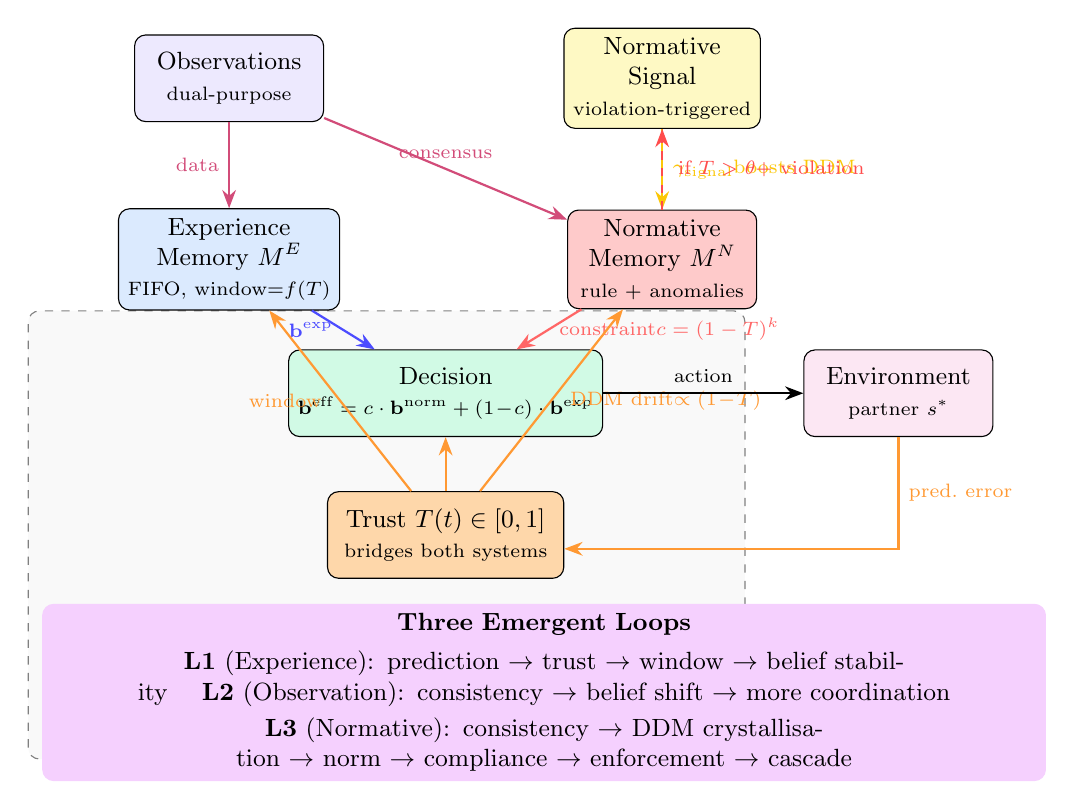
\begin{tikzpicture}[
    >=Stealth,
    box/.style={draw, rounded corners, minimum width=2.4cm, minimum height=1.1cm, align=center, font=\small},
    smallbox/.style={draw, rounded corners, minimum width=1.8cm, minimum height=0.8cm, align=center, font=\scriptsize},
    arrow/.style={->, thick},
    label/.style={font=\scriptsize, midway},
    every node/.style={font=\small}
]

% ---- Two Memory Systems ----
\node[box, fill=memblue] (expmem) at (-2, 3.5) {Experience\\Memory $M^E$\\{\scriptsize FIFO, window=$f(T)$}};
\node[box, fill=normred] (normmem) at (3.5, 3.5) {Normative\\Memory $M^N$\\{\scriptsize rule + anomalies}};

% ---- Trust ----
\node[box, fill=trustorange, minimum width=3cm] (trust) at (0.75, 0) {Trust $T(t) \in [0,1]$\\{\scriptsize bridges both systems}};

% ---- Decision ----
\node[box, fill=beliefgreen] (decision) at (0.75, 1.8) {Decision\\{\scriptsize $\mathbf{b}^{\text{eff}} = c \cdot \mathbf{b}^{\text{norm}} + (1\!-\!c) \cdot \mathbf{b}^{\text{exp}}$}};

% ---- Observations ----
\node[box, fill=commpurple] (obs) at (-2, 5.8) {Observations\\{\scriptsize dual-purpose}};

% ---- Normative Signal ----
\node[box, fill=normyellow] (signal) at (3.5, 5.8) {Normative\\Signal\\{\scriptsize violation-triggered}};

% ---- Environment ----
\node[box, fill=envpink] (env) at (6.5, 1.8) {Environment\\{\scriptsize partner $s^*$}};

% ---- Agent boundary ----
\begin{scope}[on background layer]
    \node[draw=gray, dashed, rounded corners, fill=gray!5,
          fit=(expmem)(normmem)(trust)(decision),
          inner sep=14pt, label={[font=\small\bfseries]above:AGENT}] {};
\end{scope}

% ---- Internal arrows ----
\draw[arrow, blue!70] (expmem) -- node[label, left] {$\mathbf{b}^{\text{exp}}$} (decision);
\draw[arrow, red!60] (normmem) -- node[label, right] {constraint\\{\scriptsize $c=(1-T)^k$}} (decision);
\draw[arrow, orange!80] (trust) -- node[label, left, xshift=-3pt] {window} (expmem);
\draw[arrow, orange!80] (trust) -- node[label, right, xshift=3pt] {DDM drift\\{\scriptsize $\propto(1\!-\!T)$}} (normmem);
\draw[arrow, orange!80] (trust) -- (decision);

% ---- Environment arrows ----
\draw[arrow] (decision) -- node[label, above] {action} (env);
\draw[arrow, orange!80] (env) |- node[label, near start, right] {pred.\ error} ([yshift=-5pt]trust.east);

% ---- Observation arrows ----
\draw[arrow, purple!70] (obs) -- node[label, left] {data} (expmem);
\draw[arrow, purple!70] (obs) -- node[label, above] {consensus} (normmem);

% ---- Signal arrows ----
\draw[arrow, yellow!60!orange, thick] (signal) -- node[label, right] {$\gamma_{\text{signal}}$\\{\scriptsize boosts DDM}} (normmem);

% ---- Enforcement arrow (from decision out) ----
\draw[arrow, red!70, dashed] (normmem) -- node[label, right, xshift=2pt] {if $T>\theta$\\+ violation} (signal);

% ---- Lock-in annotation ----
\node[draw=lockinpink, fill=lockinpink, rounded corners, text width=12.5cm, align=center, font=\small] at (2, -2) {
    \textbf{Three Emergent Loops}\\[3pt]
    \textbf{L1} (Experience): prediction $\to$ trust $\to$ window $\to$ belief stability \quad
    \textbf{L2} (Observation): consistency $\to$ belief shift $\to$ more coordination\\[2pt]
    \textbf{L3} (Normative): consistency $\to$ DDM crystallisation $\to$ norm $\to$ compliance $\to$ enforcement $\to$ cascade
};

\end{tikzpicture}
\caption{Dual-memory architecture. Trust bridges experience memory (statistical, FIFO) and normative memory (rule-based, anomaly-tracked). Observations feed both systems simultaneously. Normative signals are violation-triggered and confidence-gated, accelerating DDM crystallisation in receivers.}
\label{fig:dual_memory}
\end{figure}

% =====================================================================
\section{Summary}
% =====================================================================

\subsection*{The Model in One Paragraph}

Agents maintain two memory systems bridged by trust. \textbf{Experience memory} stores interaction history in a trust-modulated sliding window, producing statistical beliefs; this creates \emph{cognitive lock-in} where successful coordination stabilises beliefs through expanded memory. \textbf{Normative memory} stores internalised rules as decision constraints, formed through a stochastic drift-diffusion process \citep{germar2019learning} when uncertain agents observe consistent behaviour. Once formed, norms are maintained through anomaly accumulation (not statistical updating) and overthrown only through crisis-induced phase transitions. Trust determines whether an agent is a \emph{norm receiver} (low trust $\to$ internalise others' consistency as a rule), a \emph{norm follower} (medium trust $\to$ comply with the constraint), or a \emph{norm enforcer} (high trust $\to$ broadcast normative signals when violations are observed). The three feedback loops---cognitive lock-in, social amplification, and normative pressure---emerge naturally from this architecture. The result: a model where experience memory explains norm \emph{stability}, normative memory explains norm \emph{prescriptive force}, and their interaction through trust produces self-enforcing social norms from cold start.

\subsection*{Key Equations}

\begin{align*}
\text{Experience belief:} && b_A &= n_A / |M'^E| && \text{(statistical)} \\
\text{Trust:} && T^* &= p\alpha / (p\alpha + (1\!-\!p)\beta) && \text{(steady state)} \\
\text{Window:} && w &= \text{base} + \lfloor T(\text{max} - \text{base}) \rfloor && \text{(lock-in)} \\
\text{DDM:} && e(t\!+\!1) &= e(t) + (1\!-\!T) \cdot \text{consistency} + \mathcal{N}(0,\sigma^2) && \text{(norm formation)} \\
\text{Compliance:} && c &= (1 - T)^k && \text{(norm constraint)} \\
\text{Decision:} && \mathbf{b}^{\text{eff}} &= c \cdot \mathbf{b}^{\text{norm}} + (1\!-\!c) \cdot \mathbf{b}^{\text{exp}} && \text{(integration)} \\
\text{Enforcement:} && & T > \theta_{\text{enforce}} \,\wedge\, s^* \neq r \;\Rightarrow\; \text{broadcast}(r) && \text{(violation-triggered)}
\end{align*}

% =====================================================================
\bibliographystyle{apalike}
\begin{thebibliography}{99}

\bibitem[Behrens et al.(2007)]{behrens2007learning}
Behrens, T.~E.~J., Woolrich, M.~W., Walton, M.~E., \& Rushworth, M.~F.~S. (2007).
Learning the value of information in an uncertain world.
\textit{Nature Neuroscience}, 10(9), 1214--1221.

\bibitem[Bicchieri(2006)]{bicchieri2006grammar}
Bicchieri, C. (2006).
\textit{The Grammar of Society: The Nature and Dynamics of Social Norms}.
Cambridge University Press.

\bibitem[Centola et al.(2018)]{centola2018tipping}
Centola, D., Becker, J., Brackbill, D., \& Baronchelli, A. (2018).
Experimental evidence for tipping points in social convention.
\textit{Science}, 360(6393), 1116--1119.

\bibitem[Chudek \& Henrich(2011)]{chudek2011culture}
Chudek, M., \& Henrich, J. (2011).
Culture--gene coevolution, norm-psychology and the emergence of human prosociality.
\textit{Trends in Cognitive Sciences}, 15(5), 218--226.

\bibitem[Cialdini \& Goldstein(2004)]{cialdini2004social}
Cialdini, R.~B., \& Goldstein, N.~J. (2004).
Social influence: Compliance and conformity.
\textit{Annual Review of Psychology}, 55, 591--621.

\bibitem[Deutsch \& Gerard(1955)]{deutsch1955study}
Deutsch, M., \& Gerard, H.~B. (1955).
A study of normative and informational social influences upon individual judgment.
\textit{Journal of Abnormal and Social Psychology}, 51(3), 629--636.

\bibitem[Fehr \& Fischbacher(2004)]{fehr2004third}
Fehr, E., \& Fischbacher, U. (2004).
Third-party punishment and social norms.
\textit{Evolution and Human Behavior}, 25(2), 63--87.

\bibitem[Fehr \& G\"{a}chter(2000)]{fehr2000cooperation}
Fehr, E., \& G\"{a}chter, S. (2000).
Cooperation and punishment in public goods experiments.
\textit{American Economic Review}, 90(4), 980--994.

\bibitem[Fehr \& G\"{a}chter(2002)]{fehr2002altruistic}
Fehr, E., \& G\"{a}chter, S. (2002).
Altruistic punishment in humans.
\textit{Nature}, 415, 137--140.

\bibitem[Germar et al.(2014)]{germar2014social}
Germar, M., Schlemmer, A., Krug, K., Voss, A., \& Mojzisch, A. (2014).
Social influence and perceptual decision making: A diffusion model analysis.
\textit{Personality and Social Psychology Bulletin}, 40(2), 217--231.

\bibitem[Germar \& Mojzisch(2019)]{germar2019learning}
Germar, M., \& Mojzisch, A. (2019).
Learning of social norms can lead to a persistent perceptual bias: A diffusion model approach.
\textit{Journal of Experimental Social Psychology}, 80, 8--16.

\bibitem[Henrich \& Boyd(1998)]{henrich1998conformist}
Henrich, J., \& Boyd, R. (1998).
The evolution of conformist transmission and the emergence of between-group differences.
\textit{Evolution and Human Behavior}, 19(4), 215--241.

\bibitem[Hertwig \& Pleskac(2010)]{hertwig2010decisions}
Hertwig, R., \& Pleskac, T.~J. (2010).
Decisions from experience: Why small samples?
\textit{Cognition}, 115(2), 225--237.

\bibitem[Hume(1739)]{hume1739treatise}
Hume, D. (1739).
\textit{A Treatise of Human Nature}.

\bibitem[Kuhn(1962)]{kuhn1962structure}
Kuhn, T.~S. (1962).
\textit{The Structure of Scientific Revolutions}.
University of Chicago Press.

\bibitem[Nevo \& Erev(2012)]{nevo2012bi}
Nevo, I., \& Erev, I. (2012).
Bounded memory, inertia, sampling and weighting model for market entry games.
\textit{Games}, 3(1), 20--41.

\bibitem[Rendell et al.(2010)]{rendell2010copy}
Rendell, L., Boyd, R., Cownden, D., et al. (2010).
Why copy others? Insights from the social learning strategies tournament.
\textit{Science}, 328(5975), 208--213.

\bibitem[Sanborn \& Chater(2016)]{sanborn2016bayesian}
Sanborn, A.~N., \& Chater, N. (2016).
Bayesian brains without probabilities.
\textit{Trends in Cognitive Sciences}, 20(12), 883--893.

\bibitem[Sherif(1936)]{sherif1936psychology}
Sherif, M. (1936).
\textit{The Psychology of Social Norms}.
Harper.

\bibitem[Skitka(2010)]{skitka2010moral}
Skitka, L.~J. (2010).
The psychology of moral conviction.
\textit{Social and Personality Psychology Compass}, 4(4), 267--281.

\bibitem[Slovic(1993)]{slovic1993perceived}
Slovic, P. (1993).
Perceived risk, trust, and democracy.
\textit{Risk Analysis}, 13(6), 675--682.

\bibitem[Tenenbaum et al.(2011)]{tenenbaum2011grow}
Tenenbaum, J.~B., Kemp, C., Griffiths, T.~L., \& Goodman, N.~D. (2011).
How to grow a mind: Statistics, structure, and abstraction.
\textit{Science}, 331(6022), 1279--1285.

\bibitem[Toelch \& Dolan(2015)]{toelch2015informational}
Toelch, U., \& Dolan, R.~J. (2015).
Informational and normative influences in conformity from a neurocomputational perspective.
\textit{Trends in Cognitive Sciences}, 19(10), 579--589.

\bibitem[Toribio-Fl\'{o}rez et al.(2023)]{toribio2023proof}
Toribio-Fl\'{o}rez, D., Sasse, J., \& Baumert, A. (2023).
Proof under reasonable doubt: Ambiguity of the norm violation as boundary condition of third-party punishment.
\textit{Personality and Social Psychology Bulletin}, 49(3).

\bibitem[Toyokawa et al.(2019)]{toyokawa2019conformist}
Toyokawa, W., Whalen, A., \& Laland, K.~N. (2019).
Social learning strategies regulate the wisdom and madness of interactive crowds.
\textit{Nature Human Behaviour}, 3(2), 183--193.

\bibitem[Young(1993)]{young1993evolution}
Young, H.~P. (1993).
The evolution of conventions.
\textit{Econometrica}, 61(1), 57--84.

\end{thebibliography}

\end{document}
